\documentclass[Main]{subfiles}
\begin{document}

\chapter{Generel beskrivelse}
Dette afsnit giver et overblik over kravene, der er stillet for udviklingen af systemet.

\section{Systembeskrivelse}
Projektet vil bestå i at få en drone til, at udføre nogle specifikke programsekvenser, der styres af en bruger vha. en fjernbetjening.
Dronen har indbygget en radio, der modtager et programsignal fra fjernbetjeningen, som dronen derefter eksekverer.
\\
Dronen er foruden dette selvstabiliserende og holder sig derfor i luften og har indbygget sensorer på sin front, der i samspil med dronens software sørger for den ikke flyver ind i objekter.


\subsection{Systemoversigt}

\begin{figure}[H]
\centering
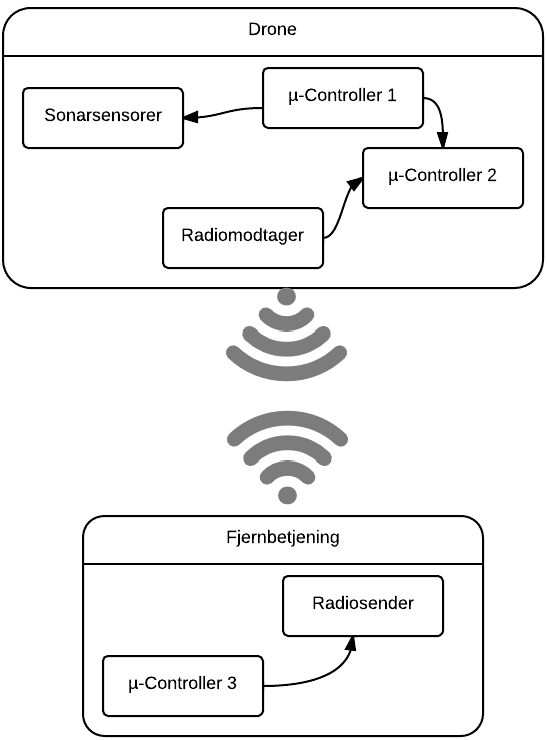
\includegraphics[scale=0.5]{Oversigt}
\caption{Systemoversigt}
\label{Fig:Oversigt}
\end{figure}

På Figur \ref{Fig:Oversigt} ses det samlede system med kommunikationen mellem dronen og fjernbetjeningen.
Fjernbetjeningen modtager et input fra nogle knapper, processerer dette i µ-Controller 3 og gennem radiosenderen overføres programvalget til dronens radiomodtager.
Herefter bearbejder µ-Controller 2 signalet og klargører dette til µ-Controller 1.
Når µ-Controller 1 skal bruge input fra fjernbetjeningen aflæses dette, samtidig med input fra sonarsensorerne.



\subsection{Aktør-kontekst diagram}

På Figur \ref{Fig:Aktor-oversigt} vises aktørerne der kommunikerer med systemet.
Figuren indeholder to grupper, henholdsvis brugeren og hardware aktører.


\begin{figure}[H]
\centering
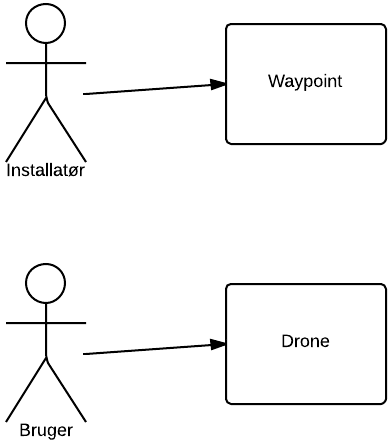
\includegraphics[scale=0.5]{AktQrDiagram}
\caption{Aktør-kontekst diagram}
\label{Fig:Aktor-oversigt}
\end{figure}


\subsection{Aktørbeskrivelser}
I det følgende beskrives aktøren, hvis opgave ønskes opfyldt af systemets Use Cases. 

\begin{longtable}{p{0.3\textwidth}|p{0.65\textwidth}}
\hline
\textbf{Aktør navn}  				& Bruger \\
\textbf{Type} 						& Primær \\
\textbf{Beskrivelse} 				& En bruger er en person, der starter, manøvrerer og stopper dronen. \\
\textbf{Antal samtidige aktører} 	& 1 \\
\hline
\end{longtable}

\begin{longtable}{p{0.3\textwidth}|p{0.65\textwidth}}
\hline
\textbf{Aktør navn}  				& Drone \\
\textbf{Type} 						& Sekundær \\
\textbf{Beskrivelse} 				& Dronen består af AeroQuad Cyclone ARF Kit, fire sonarsensorer samt 3 FM-transceivere. \\
\textbf{Antal samtidige aktører} 	& 1 \\
\hline
\end{longtable}


\section{Systemets funktioner}
Systemets funktioner, de funktionelle krav, er fundet og beskrevet vha. Use Case teknikken. 
De følgende diagrammer viser systemets funktioner udtrykt som Use Cases. 
Formålet med disse diagrammer er at give et overblik over funktionaliteten i det system, der skal udvikles. 
Hver af de på diagrammerne viste Use Cases er detaljeret specificeret i kapitel \dots \fxnote{Kapitel 3}.



\subsection{Use Case diagrammer}
Figur \ref{Fig:UC-Diagram} viser systemet som Use Case diagram.

\begin{figure}[hbtp]
\centering
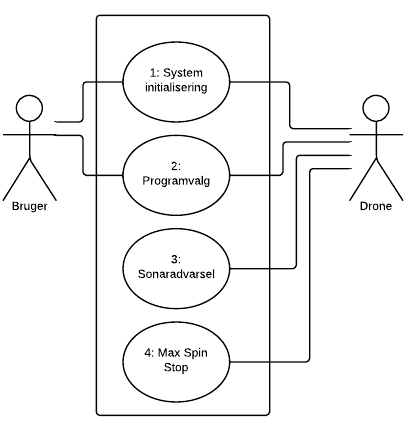
\includegraphics[scale=0.75]{UseCaseDiagram}
\caption{Use Case diagram}
\label{Fig:UC-Diagram}
\end{figure}


\end{document}